% Preamble
\documentclass[a4paper, 12pt]{article}
\usepackage[margin=1in]{geometry} % Set margin
\usepackage{pdfpages} % Insert pdf pages
\usepackage{amssymb,amsmath,amsthm, amsfonts} % Math libraries


% Custom commands
\newcommand{\sub}[1]{\subsection{\underline{#1}}}
\newcommand{\subsub}[1]{\subsubsection{\underline{#1}}}
\newcommand{\?}{\stackrel{?}{=}}
\newcommand{\R}{\ensuremath{\mathbb{R}}}
\newcommand{\F}{\ensuremath{\mathbb{F}}}
\newcommand{\eqbcuz}[1]{\text{~$\stackrel{(#1)}{=}$~}}
\renewcommand{\qed}{$$\blacksquare$$}
\renewcommand{\b}[1]{\textbf{#1}}
\renewcommand{\because}[1]{~\b{(#1)}\\}
\renewcommand{\d}{\ensuremath{\Downarrow\\~}}

% Begin Document %
\begin{document}

% Title Page
\begin{titlepage}
    %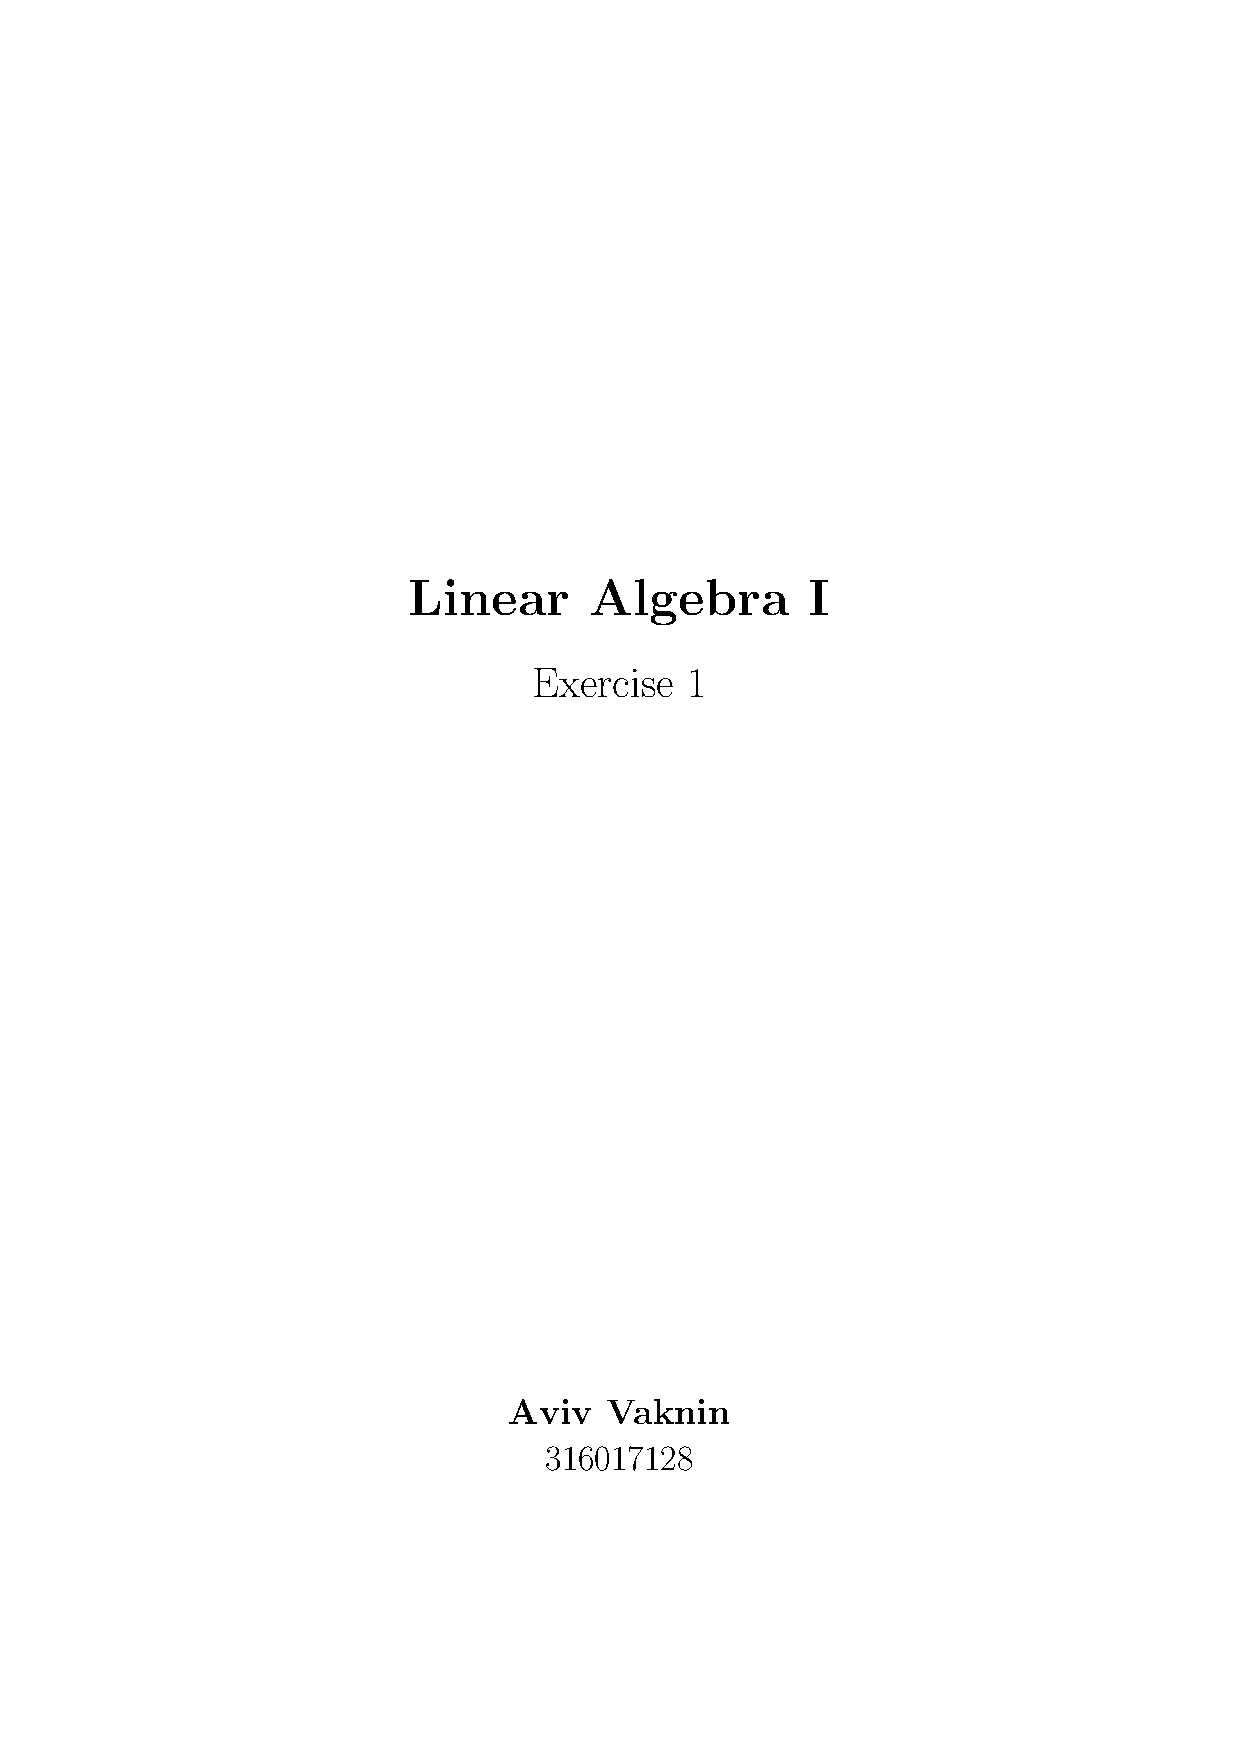
\includepdf{title.pdf}
\end{titlepage}

% 1
\section{What requirements S must fullfil in order to become a field?}
    In order to show that $S$ is a field, we'll need to prove the following \textit{\textbf{binary operator}} properties:
    \begin{enumerate}
        \item In $S$, there are two members, zero - $0_S$ and one - $1_S$
        \item $S$ supports the addition and multiplication binary operators
        \item Every member in $S$ can be negated, i.e. for every $x$ there is $-x$
        \item For every member in $S$ that is not $0_S$, $\exists{x^{-1}}\in{S}$, it is called the multiplicative inverse of $x$
    \end{enumerate}
    In addition, the mentioned binary operators should satisfy the following properties, referred to as \textit{\textbf{field axioms}}:
    \begin{enumerate}
        \item Associativity of addition(A1) and multiplication(M1):
            $$ a+(b+c)=(a+b)+c $$
            $$ a\cdot(b\cdot{c})=(a\cdot{b})\cdot{c} $$
        \item Commutativity of addition(A2) and multiplication(M2):
            $$ a+b = b+a $$
            $$ a\cdot{b} = b\cdot{a} $$
        \item Additive identity(A3) and multiplicative identity(M3)
            $$ a+0=a $$
            $$ a\cdot{1}=a $$
        \item Additive inverse(A4) and multiplicative inverse(M4)
            $$ a + (-a) = 0 $$
            $$ a \cdot a^-1 = 1 $$
        \item Distributivity(D)
            $$ a(b + c) = (a \cdot{b})+(a \cdot{c}) $$
    \end{enumerate}
\pagebreak

% 2
\section{Prove: $ ((a + b) + c) + d = (a + b) + (c + d) = a + (b + (c + d)) $}

\sub{$((a+b)+c)+d=(a+b)+(c+d)$:}
First of all, we'll take a look at the left side of the equation.\\
We'll mark: $$h=(a+b)$$
Therefore: $$(h+c)+d=((a+b)+c)+d$$
$$(h+c)+d \eqbcuz{A1} h+(c+d) $$
We'll subtitue $h$ with $(a+b)$: $$ h+(c+d) = (a+b)+(c+d) $$
$$\d$$
$$((a+b)+c)+d=(a+b)+(c+d)$$

\sub{$a+(b+(c+d))=(a+b)+(c+d)$:}
We'll mark: $$h=(c+d)$$
Therefore: $$ a+(b+h) = a+(b+(c+d)) $$
$$ a+(b+h) \eqbcuz{A1} (a+b)+h $$
We'll subtitue $h$ with $(c+d)$: $$ (a+b)+h = (a+b)+(c+d) $$
$$\d$$
$$ a+(b+(c+d)) = (a+b)+(c+d) $$
\qed

% 3
\section{Prove: $ \forall{x,y}\in{F},~x(y-z) = xy-xz $}
$ x(y-z) = x(y+(-z)) $\because{A1}
$ x(y+(-z)) = (x\cdot{y})+(x\cdot(-z))$\because{D}
$ (x\cdot{y})+(x\cdot(-z)) = (x\cdot{y})+(-x\cdot{z})) = (x\cdot{y})-(x\cdot{z})) $\\
$ (x\cdot{y})-(x\cdot{z})) = xy - xz $\\
\qed

% 4
\section{Prove: $ \forall{x,y}\in{F},~ (x+y)(x+y) = xx + xy + yx + yy $}
let $ h=(x+y) $
$
    (x+y)(x+y) = h\cdot(x+y)\\
    h\cdot(x+y) = (x\cdot{h})+(y\cdot{h}) = x(x+y) + y(x+y) \because{D}
    x(x+y) + y(x+y) = xx + xy + yx + yy \because{D}
$
\qed

% 5
\section{Prove: $ \forall{x,y}\in{F},~ (x+y)(x-y) = xx - yy $}

$
    (x+y)(x-y) = xx - xy + yx - yy \because{ex. 4}
    xx - xy + yx - yy = xx + (-xy + yx) - yy \because{A1}
    (-xy + yx) = (-xy + xy) \because{A2}
    (-xy + xy) = 0 \because{A4}
    \d
    xx + (-xy + yx) - yy = xx + 0 - yy = xx - yy \because{A3}
$
\qed

% 6
\section{Prove: $ (a=b) \land (c=d) \Rightarrow (a+c=b+d) \land (ac=bd) $}

\sub{$ (a=b) \land (c=d) \Rightarrow a+c=b+d $:}
$
    c=d=x \\
    a=b \\
    a+x=b+x \because{Consistency with addition}
    a+x=a+c \because{x=c}
    b+x=b+d \because{x=d}
    \d
    a+c=b+d\\
$

\sub{$ (a=b) \land (c=d) \Rightarrow ac=bd $:}
$
    c=d=x \\
    a=b \\
    ax=bx \because{Consistency with multiplication}
    ax=ac \because{x=c}
    bx=bd \because{x=d}
    \d
    ac=bd\\
$
\qed

% 7
\section{$ A=\bigg{\{} \dbinom{1}{a} \bigg{|} a\in{\R}\bigg{\}} $}
    \sub{Does A have a neutral additive member?}
    $
        \dbinom{1}{a} \oplus \dbinom{1}{0} = \dbinom{1}{a+0} \\
        \dbinom{1}{a+0} = \dbinom{1}{a} \because{A3}
        \d
        0_{A} = \dbinom{1}{0}
    $
    \sub{Does A have a neutral multiplicative member?}
    $
        \dbinom{1}{a} \odot \dbinom{1}{1} = \dbinom{1}{a \cdot{1}} \\
        \dbinom{1}{a \cdot{1}} = \dbinom{1}{a} \because{M3}
        \d
        1_{A} = \dbinom{1}{1}
    $
    \sub{Is A a field?}
        \subsub{A1 - Additive Associativity}
        $
            \bigg{[}\dbinom{1}{a}\oplus{}\dbinom{1}{b}\bigg{]}\oplus{}\dbinom{1}{c} \? \dbinom{1}{a} \oplus{} \bigg{[}\dbinom{1}{b}\oplus{}\dbinom{1}{c}\bigg{]} \\
            \dbinom{1}{a+b}\oplus{}\dbinom{1}{c} \? \dbinom{1}{a} \oplus{} \dbinom{1}{b+c} \\
            \dbinom{1}{a+b+c} = \dbinom{1}{a+b+c} \\
            \d
            \bigg{[}\dbinom{1}{a}\oplus{}\dbinom{1}{b}\bigg{]}\oplus{}\dbinom{1}{c} = \dbinom{1}{a} \oplus{} \bigg{[}\dbinom{1}{b}\oplus{}\dbinom{1}{c}\bigg{]}
        $
        \pagebreak
        \subsub{M1 - Multiplicative Associativity}
        $
            \bigg{[}\dbinom{1}{a}\odot{}\dbinom{1}{b}\bigg{]}\odot{}\dbinom{1}{c} \? \dbinom{1}{a} \odot{} \bigg{[}\dbinom{1}{b}\odot{}\dbinom{1}{c}\bigg{]} \\
            \dbinom{1}{ab}\odot{}\dbinom{1}{c} \? \dbinom{1}{a} \odot{} \dbinom{1}{bc} \\
            \dbinom{1}{abc} = \dbinom{1}{abc} \\
            \d
            \bigg{[}\dbinom{1}{a}\odot{}\dbinom{1}{b}\bigg{]}\odot{}\dbinom{1}{c} = \dbinom{1}{a} \odot{} \bigg{[}\dbinom{1}{b}\odot{}\dbinom{1}{c}\bigg{]}
        $
        \subsub{A2 - Additive Commutativity}
        $
            \dbinom{1}{a} \oplus \dbinom{1}{b} \? \dbinom{1}{b} \oplus \dbinom{1}{a} \\
            \dbinom{1}{a+b} \? \dbinom{1}{b+a} \\
            \dbinom{1}{a+b} = \dbinom{1}{b+a} \because{A2: In A, $a\in\R$}
            \d
            \dbinom{1}{a} \oplus \dbinom{1}{b} = \dbinom{1}{b} \oplus \dbinom{1}{a}
        $
        \subsub{M2 - Multiplicative Commutativity}
        $
            \dbinom{1}{a} \odot \dbinom{1}{b} \? \dbinom{1}{b} \odot \dbinom{1}{a} \\
            \dbinom{1}{ab} \? \dbinom{1}{ba} \\
            \dbinom{1}{ab} = \dbinom{1}{ba} \because{M2: In A, $a\in\R$}
            \d
            \dbinom{1}{a} \odot \dbinom{1}{b} = \dbinom{1}{b} \odot \dbinom{1}{a}
        $
        \subsub{A3 - Additive Identity}
        $
            \exists\dbinom{1}{a},\dbinom{1}{b}\in{A}\bigg{|}\dbinom{1}{a}\oplus\dbinom{1}{b}=\dbinom{1}{a}? \\
            \dbinom{1}{a}\oplus\dbinom{1}{0}=\dbinom{1}{a+0}=\dbinom{1}{a} \because{A3: In A, $a\in\R$}
            \d
            \dbinom{1}{0} = 0_{A}
        $
        \pagebreak
        \subsub{M3 - Multiplicative Identity}
        $
            \exists\dbinom{1}{a},\dbinom{1}{b}\in{A}\bigg{|}\dbinom{1}{a}\odot\dbinom{1}{b}=\dbinom{1}{a}? \\
            \dbinom{1}{a}\odot\dbinom{1}{1}=\dbinom{1}{1a}=\dbinom{1}{a} \because{M3: In A, $a\in\R$}
            \d
            \dbinom{1}{1} = 1_{A}
        $
        \subsub{A4 - Additive Inverse}
        $
            \exists\dbinom{1}{a},\dbinom{1}{b}\in{A}\bigg{|}\dbinom{1}{a}\oplus\dbinom{1}{b}=0_{A}? \\
            \dbinom{1}{a}\oplus\dbinom{1}{-a}=\dbinom{1}{a+(-a)}=\dbinom{1}{0}=0_{A} \because{A4: In A, $a\in\R$}~
        $
        \subsub{M4 - Multiplicative Inverse}
        $
            \exists\dbinom{1}{a},\dbinom{1}{b}\in{A}\bigg{|}\dbinom{1}{a}\odot\dbinom{1}{b}=1_{A}? \\
            \dbinom{1}{a}\odot\dbinom{1}{\frac{1}{a}}=\dbinom{1}{a\cdot{\frac{1}{a}}} \\
            \dbinom{1}{a\cdot{\frac{1}{a}}} = \dbinom{1}{\frac{a}{a}} \\
            \dbinom{1}{\frac{a}{a}} = \dbinom{1}{1} = 1_{A}
        $
        \subsub{D - Distributivity}
        In order to display distributivity, we'll need to show the A equivalent of:
        $$ a\cdot{(b+c)}=a\cdot{b}+a\cdot{c} $$
        We need to prove: $ \dbinom{1}{a} \odot \bigg{[} \dbinom{1}{b} \oplus \dbinom{1}{c} \bigg{]} \? \dbinom{1}{ab} \oplus \dbinom{1}{ac} $ \\
        A's Addition property: $ \dbinom{1}{a} \odot \bigg{[} \dbinom{1}{b} \oplus \dbinom{1}{c} \bigg{]} = \dbinom{1}{a} \odot \dbinom{1}{b+c} $ \\
        A's Multiplication property: $ \dbinom{1}{a} \odot \dbinom{1}{b+c} = \dbinom{1}{a(b+c)} $ \\
        Since A's bottom member of the pair $\in{\R}$, we'll use Axiom D:
        $$ \dbinom{1}{a(b+c)} = \dbinom{1}{ab} \oplus \dbinom{1}{ac} $$
        \qed\pagebreak

% 8
\section{Is $B$ a field?}
    If $B$ fulfills all 9 field's axioms, $B$ is a field, let's check them one by one.
    \sub{A1 - Additive Associativity}
        $$ \bigg{[}\dbinom{a}{b}\oplus{}\dbinom{c}{d}\bigg{]}\oplus{}\dbinom{e}{f} \? \dbinom{a}{b} \oplus{} \bigg{[}\dbinom{c}{d}\oplus{}\dbinom{e}{f}\bigg{]} $$
        $$ \dbinom{a+c}{b+d}\oplus{}\dbinom{e}{f} \? \dbinom{a}{b} \oplus{} \dbinom{c+e}{d+f} $$
        $$ \dbinom{a+c+e}{b+d+f} = \dbinom{a+c+e}{b+d+f} $$

    \sub{M1 - Multiplicative Associativity}
        $$ \bigg{[}\dbinom{a}{b}\odot{}\dbinom{c}{d}\bigg{]}\odot{}\dbinom{e}{f} \? \dbinom{a}{b} \odot{} \bigg{[}\dbinom{c}{d}\odot{}\dbinom{e}{f}\bigg{]} $$
        $$ \dbinom{ac}{bd}\odot{}\dbinom{e}{f} \? \dbinom{a}{b} \odot{} \dbinom{ce}{df} $$
        $$ \dbinom{ace}{bdf} = \dbinom{ace}{bdf} $$

    \sub{A2 - Additive Commutativity}
        $$ \dbinom{a}{b} \oplus \dbinom{c}{d} \? \dbinom{c}{d} \oplus \dbinom{a}{b} $$
        $$ \dbinom{a+c}{b+d} \? \dbinom{c+a}{d+b} $$
        As $a,b \in {\R}$, we can use axiom A2:
        $$ \dbinom{a+c}{b+d} = \dbinom{c+a}{d+b} $$

    \sub{M2 - Multiplicative Commutativity}
        $$ \dbinom{a}{b} \odot \dbinom{c}{d} \? \dbinom{c}{d} \odot \dbinom{a}{b} $$
        $$ \dbinom{ac}{bd} \? \dbinom{ca}{db} $$
        As $a,b,c,d \in {\R}$, we can use axiom M2:
        $$ \dbinom{ac}{bd} = \dbinom{ca}{db} $$

    \sub{A3 - Additive Identity}
        Now, we'll look for $0_{B}$:
        $$ \dbinom{a}{b}\oplus\dbinom{0}{0} = \dbinom{a+0}{b+0} $$
        As $a,b \in {\R}$, we can use axiom A3:
        $$ \dbinom{a+0}{b+0} = \dbinom{a}{b} $$
        Therefore:
        $$ \dbinom{0}{0} = 0_{B} $$
    
    \sub{M3 - Multiplicative Identity}
        Now, we'll look for $1_{B}$:
        $$ \dbinom{a}{b}\odot\dbinom{1}{1} = \dbinom{1a}{1b} $$
        As $a,b \in {\R}$, we can use axiom M3:
        $$ \dbinom{1a}{1b} = \dbinom{a}{b} $$ 
        Therefore:
        $$ \dbinom{1}{1} = 1_{B} $$

    \sub{A4 - Additive Inverse}
        Now, let us find if exists a member, $\dbinom{c}{d} \in{B}$, for any other member $\dbinom{a}{b} \in{B}$, so that:
        $$ \dbinom{a}{b}\oplus\dbinom{c}{d} = 0_{B} $$
        We'll start by adding the inverse of every number to itself:
        $$\dbinom{a}{b}\oplus\dbinom{-a}{-b} = \dbinom{a+(-a)}{b+(-b)} $$
        As $a,b \in {\R}$, we can use axiom A4 to find the sum's value:
        $$ \dbinom{a+(-a)}{b+(-b)} =\dbinom{0}{0}=0_{B} $$
        \pagebreak

    \sub{M4 - Multiplicative Inverse}
        Now, let us find if exists a member, $\dbinom{c}{d} \in{B}$, for any other member $\dbinom{a}{b} \in{B}$, so that:
        $$ \dbinom{a}{b}\odot\dbinom{c}{d} = 1_{B} $$
        Let's multiply every number by its multiplicitive inverse:
        $$ \dbinom{a}{b}\odot\dbinom{\frac{1}{a}}{\frac{1}{b}}=\dbinom{a\cdot{\frac{1}{a}}}{b\cdot{\frac{1}{b}}} $$
        As $a,b \in {\R}$, we can use axiom M4:
        $$ \dbinom{a\cdot{\frac{1}{a}}}{b\cdot{\frac{1}{b}}} = \dbinom{1}{1} $$
        $$ \dbinom{1}{1} = 1_{B} $$

    \sub{D - Distributivity}
    In order to display distributivity, we'll need to show the $B$ equivalent of:
    $$ a\cdot{(b+c)}=a\cdot{b}+a\cdot{c} $$
    i.e., we need to prove:
    $$ \dbinom{a}{b} \odot \bigg{[} \dbinom{c}{d} \oplus \dbinom{e}{f} \bigg{]} = \dbinom{ac}{bd} \oplus \dbinom{ae}{bf} $$
    First, let's solve: $$ \bigg{[} \dbinom{c}{d} \oplus \dbinom{e}{f} \bigg{]} $$
    We use $B$'s binary additive operator:
    $$ \dbinom{c}{d} \oplus \dbinom{e}{f} = \dbinom{c+e}{d+f} $$
    We use $B$'s binary multiplicative operator: $$ \dbinom{a}{b} \odot \dbinom{c+e}{d+f} = \dbinom{a(c+e)}{b(d+f)} $$
    As $a,b,c,d,e,f \in {\R}$, we can use the distributivity axiom to unpack:
    $$ \dbinom{a(c+e)}{b(d+f)} = \dbinom{ac+ae}{bd+bf} = \dbinom{ac}{bd} \oplus \dbinom{ae}{bf} $$
    \qed
    \pagebreak

% End Document %
\end{document}